\documentclass[tikz, border=2mm]{standalone}
\usepackage{tikz}
\usetikzlibrary{calc}
\usetikzlibrary{arrows.meta}
\begin{document}
    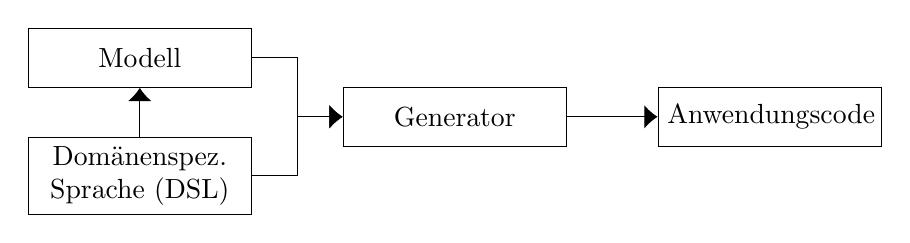
\begin{tikzpicture}
        \node[text width=2.6cm, align=center, minimum height=0.75cm] at (0,0) [rectangle,draw] (modell) {Modell};
        \node[text width=2.6cm, align=center, minimum height=0.75cm] at (4,-0.75) [rectangle,draw] (generator) {Generator};
        \node[text width=2.6cm, align=center, minimum height=0.75cm] at (8,-0.75) [rectangle,draw] (awcode) {Anwendungscode};
        \node[text width=2.6cm, align=center, minimum height=0.75cm] at (0,-1.5) [rectangle,draw] (dsl) {Dom\"anenspez. Sprache (DSL)};
        \draw[-{Latex[width=3mm]}] (modell) -- ($(modell)+(2,0)$) |- (generator);
        \draw[-{Latex[width=3mm]}] (dsl) -- (modell);
        \draw[-{Latex[width=3mm]}] (generator) -- (awcode);
        \draw[-{Latex[width=3mm]}] (dsl) -- ($(dsl)+(2,0)$) |- (generator);
    \end{tikzpicture}
\end{document}